\clearpage
\section{Soft- und Firmware}\label{sec:Soft-undFirmware}


Im folgenden Abschnitt werden Anforderungen, Konzept, Entscheidung und die Umsetzung der Software dokumentiert. Die Lösungsfindung und ihre Prozess wird nachfolgend beschrieben. 

\subsection{Anforderungen}\label{subsec:Software_Anforderungen}

Wie bereits im Abschnitt \ref{sec:Abgrenzung} wurden die Anforderungen in der Aufgabenstellung (siehe Anhang \ref{app:Aufgabenstellung}) sowie im Pflichtenheft (siehe Anhang \ref{app:Pflichtenheft}) vorgängig festgelegt. Im Fokus steht das erfassen der wichtigsten Messgrössen welche nachfolgend aufgeführt werden. \\

\begin{itemize}
	\item \textbf{Latenzzeit}: Bestimmung der Latenzzeit in Millisekunden zwischen den Teilnehmern. Die Genauigkeit sollte bei $+/-$1 ms liegen.  
	\item \textbf{Anzahl Hops}: Bestimmung der Anzahl Hops, über welche eine Nachricht übermittelt wird.
	\item \textbf{Datenrate}: Messen der Datenrate in Bytes/s, welche zwischen zwei Teilnehmern erreicht wurde. 
	\item \textbf{RSSI}: Erfassen des RSSI-Werts der eingehenden Pakete.
	\item \textbf{Paketverlust}: Pakete zählen, welche ihr Ziel nicht erreicht haben.  
	\item \textbf{Aktive Radio Zeit}: Erfassen der aktiven Radio-Zeit um den Energieverbrauch abschätzen zu können. 
\end{itemize}


Die Erfassung muss in allen Mesh-Netzwerken möglich sein. Um die Messresultate vergleichen zu können müssen die gleichen Ausgangslagen vorliegen, sowie die selben Messmethoden angewendet werden. 

\todo[inline]{Beschreiben der Anforderungen an die Software. Einzelne Teilprobleme Beschreiben}


\subsection{Konzept}\label{subsec:Software_Konzept}

Um die Messdaten erfassen zu können müssen alle Teilnehmer im Netzwerk eine eigenes Log führen. Dieses wird im Anschluss an eine zentrale Auswerte-Stelle übermittelt um ausgewertet zu werden (wie in Abschnitt ... beschrieben). Folgende Daten müssen pro eingehende oder gesendete Nachricht von allen Teilnehmern der Messung erfasst werden. 

\begin{itemize}
	\item \textbf{Message-ID}: Eindeutige Kennung (Laufnummer) welche beim Senden einer Nachricht mitgegeben wird. Somit können die Nachrichten anschliessend zugeordnet werden. 
	\item \textbf{Timestamp}: Erfassen der Sende- / Empfangszeit über synchronisierten Zeitwert. Relevant zur Bestimmung der Latenzzeit und Datenrate. 
	\item \textbf{Hops}: Auslesen der Anzahl Hops des Pakets beim Empfangen. Beim Senden kann dieser Wert ignoriert werden.
	\item \textbf{Source Address}: Erfassen der Teilnehmer-Addresse welcher die Nachricht sendet oder gesendet hat. Wichtig für die korrekte Zuordnung der Pakete. 
	\item \textbf{Destination Address}: Erfassen der Teilnehmer-Addresse welcher die Nachricht empfangen hat. Ebenfalls für Zuordnung der Nachrichten relevant. 
	\item \textbf{Group Address}: Erfassen der Gruppen-Adresse in welcher die Nachricht unterwegs war. Notwendig zur Erfassung des Paketverlustes. 
	\item \textbf{RSSI}: Erfassen des RSSI-Werts der eingehenden Pakete. Beim senden soll dieser Wert 0 sein. 
	\item \textbf{Paketgrösse}: Erfassen der Paketgrösse um die Datenrate zu berechnen. 
\end{itemize}

Zur Steuerung der Messungen wird eine zentrale Stelle (Master) verwendet (Wie in Abschnitt ... beschrieben). Diese soll einzelne Teilnehmer Konfigurieren, eine Messung starten, sowie die Reports  einsammeln können. 


\todo[inline]{Konzept zur Lösung der Teilprobleme grob beschreiben}


\subsection{Entscheidung}\label{subsec:Software_Entscheidung}

Zur Umsetzung der Mesh-Stacks mittles der \textit{NRF-Platform} sind folgende SDKs vorhanden: 

\begin{itemize}
	\item \textit{\textbf{nRF Connect SDK}}: Auf dem Zephyr-RTOS aufbauende SDK. Diese soll in Zukunft alle drei Mesh-Protokolle (Bluetooth-Mesh, Openthread und Zigbee) unterstützen. Wird jedoch noch nicht zum Einsatz in End-Produkten empfohlen. \cite{nordic_semi_welcome_to_the_nrf_connect_sdk_2020}
	\item \textit{\textbf{nRF SDK for Thread and Zigbee}}: Proprietäre SDK Library von Nordic Semiconductor. Thread integration mittels Openthread, Zigbee einbindung mittels ZBOSS. \cite{nordic_semi_nrf_sdk_for_thread_and_zigbee_2020}
	\item \textit{\textbf{nRF SDK for Mesh}}: Proprietäre SDK Library von Nordic Semiconductor für Bluetooth-Mesh. Ist zur Produktion freigegeben. \cite{nordic_semi_nrf_sdk_for_mesh_2020}
\end{itemize}

Die Messungen sollten trotz der verschiedenen Bibliotheken möglichst einheitlich sein, um die Vergleichbarkeit nicht zu beeinträchtigen. Daher musste ... Das Erfassen der Daten erfolgt Um eine möglichst unabhängig von der verwendeten Library zu sein wurde auf eine selbst entwickelte Kommunikation über die P2P-Testinfrastruktur gesetzt. 

\todo[inline]{Warum wurde die Software so umgesetzt?}

\todo[inline]{Tabelle der SDKs und Stacks und ihren Möglichkeiten aufzeigen. -> Gesamtheitliche Lösung mittels eigener Verwaltungsschicht und P2P}


\todo[inline]{Tabelle welche Software zu welchem Stack, Referenzen zu Parts}


\subsection{Umsetzung}\label{subsec:Software_Umsetzung}

\todo[inline]{Cyrill Text anpassen. Thread nutzt SharedLib voll}


Die Software und Firmware für die Mesh Benchmarks setzt sich aus diversen Modulen zusammen. Die Tabelle \ref{tab:UebersichtSoftware} zeigt eine Übersicht der wichtigsten Module und deren Verwendung in den 3 Benchmark Teilen: BLE Mesh, Thread und Zigbee.
Gemeinsame Module auf Firmware Ebene sind im Ordner SharedLib im Github Repository\footnotemark\ zusammengefasst.

Jene Python Scripts für das Benchmark Management stehen im gleichnamigen Ordner auf dem Github Repository zur Verfügung.
Die Stack bezogenen Implementationen der Benchmark Firmware werden in den individuellen Teilen \ref{part:BluetoothMesh}, \ref{part:Thread} und \ref{part:Zigbee} behandelt.


%\newcommand{\rotcells}[1]{%
%  \rotatebox[origin=c]{90}{ #1 }%
%}

\begin{table}
\centering
\caption{Übersicht Shared Lib und Benchmark Management Module}
\label{tab:UebersichtSoftware}
\begin{tabular}{|l|l|l|c|} 
\hline
Library & Funktion & Modul & Referenz \\ 
\hline
\multirow{8}{*}{SharedLib} & Statemachine & bm\_satemachine.c &  \\ 
\cline{2-4}
 & Timesync & bm\_timesync.c &  \\ 
\cline{2-4}
 & Control & bm\_control.c &  \\ 
\cline{2-4}
 & Report & bm\_report.c & xy \\ 
\cline{2-4}
 & Logging & bm\_log.c & xy \\ 
\cline{2-4}
 & Flash Save & bm\_flash\_save.c & xy \\ 
\cline{2-4}
 & CLI & bm\_cli.c & xy \\ 
\cline{2-4}
 & Low Layer Radio & bm\_radio.c & xy \\ 
\hline
\multicolumn{1}{l}{} & \multicolumn{1}{l}{} & \multicolumn{1}{l}{} & \multicolumn{1}{l}{} \\ 
\hline
\multirow{4}{*}{\begin{tabular}[c]{@{}l@{}}Benchmark\\Management \end{tabular}} & Flash & Flasher.py & xy \\ 
\cline{2-4}
 & Configurator & Configurator.py & xy \\ 
\cline{2-4}
 & Benchmark & \begin{tabular}[c]{@{}l@{}}Benchmark\_and\_\\Reporter.py \end{tabular} & xy \\ 
\cline{2-4}
 & Analysis & Analysis.py & xy \\ 
\hline
\multicolumn{1}{l}{} & \multicolumn{1}{l}{} & \multicolumn{1}{l}{} & \multicolumn{1}{l}{} \\ 
\hline
\multirow{2}{*}{BT Mesh} & Stack Handling & bm\_blemesh.c & \ref{sec:BTMeshUmsetzungBenchmark} \\ 
\cline{2-4}
 & Stack Configuration & bm\_config.c & \ref{sec:BTMeshUmsetzungBenchmark} \\ 
\hline
\multicolumn{1}{l}{} & \multicolumn{1}{l}{} & \multicolumn{1}{l}{} & \multicolumn{1}{l}{} \\ 
\hline
\multirow{2}{*}{Thread} &  &  & \ref{sec:ThreadUmsetzungBenchmark} \\ 
\cline{2-4}
 &  &  & \ref{sec:ThreadUmsetzungBenchmark} \\ 
\hline
\multicolumn{1}{l}{} & \multicolumn{1}{l}{} & \multicolumn{1}{l}{} & \multicolumn{1}{l}{} \\ 
\hline
\multirow{2}{*}{Zigbee} & Stack Handling & bm\_zigbee.c & \ref{sec:ZigbeeUmsetzungBenchmark} \\ 
\cline{2-4}
 & Stack Configuration & bm\_config.c & \ref{sec:ZigbeeUmsetzungBenchmark} \\
\hline
\end{tabular}
\end{table}


Sämtliche Firm- und Software Komponenten die für Mesh Benchmark sowie die P2P Testinfrastruktur nötig sind, können auf dem Github Repository zum Projekt unter folgendem \href{https://github.com/Rouben94/P6_Software}{Link\footnotemark[\value{footnote}]}  eingesehen werden.

\footnotetext{\url{https://github.com/Rouben94/P6_Software} \cite{anklin_bobst_horath_rouben94p6_software_nodate}}




\subsection{Shared Library}\label{subsec:SharedLibrary}

Die \textit{Shared Library} ist die geteilte Bibliothek zwischen allen Mesh-Stacks. Sie beherbergt alle relevanten Module um eine Messung zu Verwalten. Der jeweilige Mesh-Stack ist lediglich für das senden und empfangen von Nachrichten, sowie zum Erfassen der Messdaten zuständig. 


\begin{figure}[H]
	\centering
	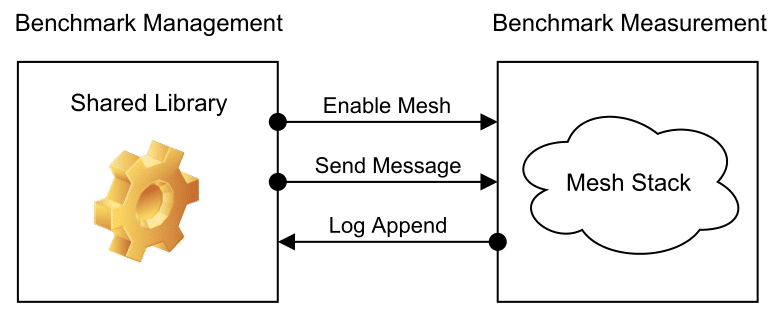
\includegraphics[width=0.6\textwidth]{Shared_Lib_Concept.png}
	\caption{Vereinfachte Anbindung der \textit{Shared Library} an die Mesh-Stacks}\label{fig:ShardeLibConcept}
\end{figure}

Abbildung \ref{fig:ShardeLibConcept} zeigt die vereinfachten Schnittstellen zwischen der Shared-Library und den Mesh-Stacks. Die Bibliothek ist spezifisch für die nRF52840 SOCs zugeschnitten. Um einfach in die jeweilige SDK integrierbar zu sein müssen die Module der Shared-Lib möglichst ohne weitere Abhängigkeiten klar kommen. Sofern Treiber oder externe Bibliotheken für Module benötigt werden, müssen diese von allen SDKs vergleichbar zur Verfügung gestellt werden. Im folgenden Abschnitt wird auf die einzelnen Module der \textit{Shared-Lib} eingegangen. 


\subsubsection{Statemachine}\label{subsubsec:StatemachineSoftware}

Die Statemachine dient dazu den Ablauf, welcher in Abschnitt \ref{subsec:AblaufMesh} beschrieben wurde abzuarbeiten. Sowohl der Master, die Server und Clients arbeiten den in Abbildung \ref{fig:StatemachineFLowgraph} dargestellten Ablauf ab. 

\begin{figure}[H]
	\centering
	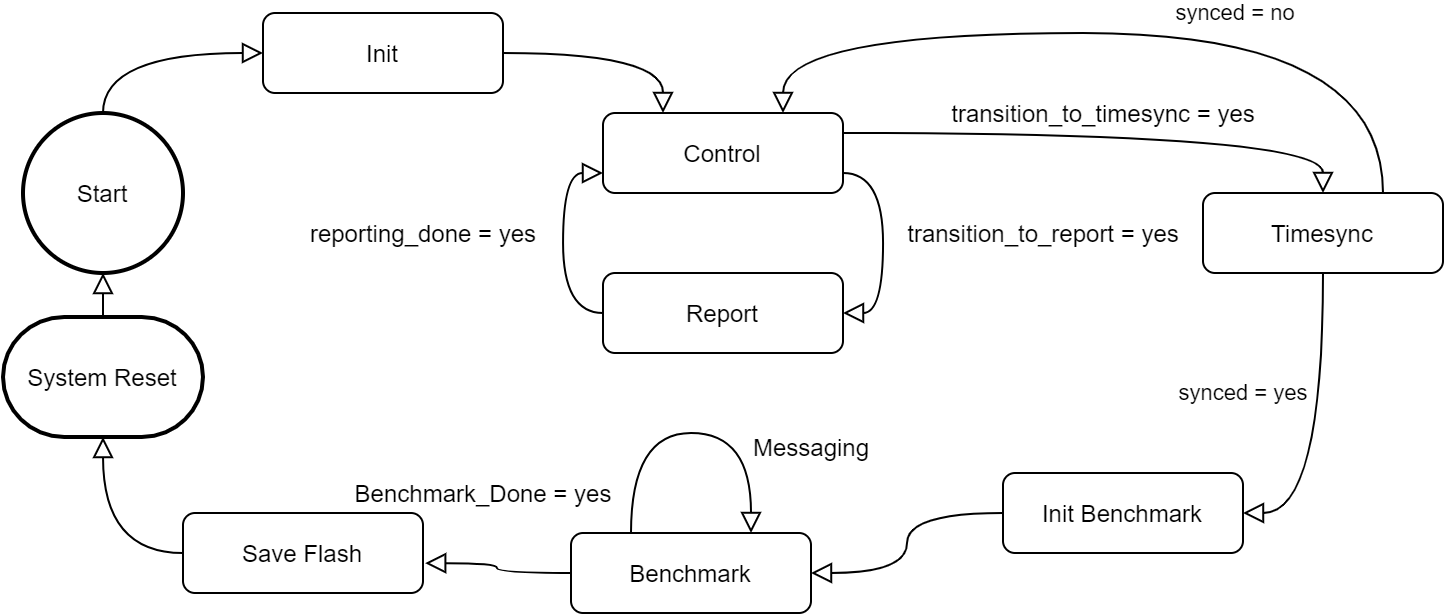
\includegraphics[width=1.0\textwidth]{Statemachine_Flowgraph.png}
	\caption{Flowgraph der Statemachine}\label{fig:StatemachineFLowgraph}
\end{figure}


Die Funktion der Schritte wird im Folgenden grob beschrieben. Zur genauen Untersuchung ist der Source Code unter \cite{rouben94_sharedlib_software_git_2020} verfügbar.  \\

\begin{itemize}
	\item \textbf{\textit{Init:}} Dieser Schritt initialisiert alle notwendige Funktionen (Radio, Timers, usw.). Ebenfalls rekonstruiert er die \textit{Log-Daten} indem er diese aus dem Flash in das RAM kopiert. Nach der erfolgreichen Initialisierung wechselt die Statemachine in den Control-State.
	\item \textbf{\textit{Control:}} Im Control-State wartet jeder Teilnehmer auf eingehende Befehle des Benutzers. Der Master erhält über das Command Line Interface (CLI) den auszuführenden Befehl. Diesen wandelt der Master in eine Nachricht (Control-Message) um und leitet sie über das Radio-Interface an die Slaves weiter.  Alle Slaves (Clients und Servers) erwarten eine Control-Message über das Radio-Interface. Damit alle Clients und Servers die Nachricht empfangen können wiederholt jeder Slave jede Control-Message. Somit wird die Mesh-Fähigkeit der Verwaltungsschicht (Benchmark Managment) sichergestellt. Folgende Transitionen sind vom Control-State zugelassen: 
	\begin{itemize}
		\item \textit{\textbf{Transition to Timesync}}: Wird ein Benchmark gestartet erfolgt dies durch einen Wechsel in den Timesync-State. Jeder Teilnehmer wechselt nach wiederholen der Nachricht in den entsprechenden Schritt. 
		\item \textit{\textbf{Transition to Report}}: Das Reporting wird über den Report-State abgehandelt. Nur der Teilnehmer von welchem Reports angefordert wurden, wechselt in den Report-State. 
	\end{itemize} 	
	\item \textbf{\textit{Timesync:}} Der Master verteilt die Zeitsynchronisation an die Slaves. Die Slaves synchronisieren sich auf das Signal des Masters auf, sofern sie in seiner Reichweite liegen. Sobald ein Slave synchronisiert ist, fängt er an die Zeitsynchronisation ebenfalls zu verteilen. Dadurch können Slaves, welche nicht über einen Hop vom Master erreicht werden sich ebenfalls synchronisieren. Konnte ein Slave keine Zeitsynchronisation durchführen, wechselt dieser in den  \textit{Control-State} zurück und bringt einen Fehler mittels der roten-LED zur Anezige. Der Master wird immer zum nächsten Schritt voranschreiten. 	
	\item \textbf{\textit{Init Benchmark:}} Dies ist der Zeitpunkt bei welchem jeder Teilnehmer den Mesh Stack-Initialisiert und Anschliessend Startet. Das Netzwerk hat nun Zeit sich aufzubauen, falls dies notwendig ist. Vor dem Initialisieren des Mesh-Stacks löscht jeder Node die Log-Daten aus dem Flash, sowie dem RAM. Beim Client wird zusätzlich der Sendezeitpunkt der Benchmark-Nachrichten (Benchmark-Messages) berechnet und vorbereitet. Hat sich der Slave erfolgreich Initialisiert und mit dem Netzwerk verbunden, beginnt das grüne Status-LED zu leuchten. Der wechsel zum Benchmark-State wird unabhängig vom Verbindungsstatus nach einer Verzögerungszeit ausgelöst. 
	\item \textbf{\textit{Benchmark:}} Die Statemachine wartet in diesem Schritt lediglich auf das auslösen von Events. Beim Server überlässt sie dem Mesh-Stack das Loggen der empfangenen Nachrichten, welcher über einen eigenen Event-Handler verfügt. Beim Client plant die Statemachine das senden von Nachrichten mittels Timer-Interrupts. Löst ein solcher aus, wird der Mesh-Stack sofort benachrichtigt. Das erfassen des Logs erfolgt ebenfalls im Stack. Der Status des einzelnen Slaves (Licht EIN / Aus) ist über die grüne RGB-LED (Client) oder die blaue RGB-LED (Server) erkennbar. Nach der eingestellten Benchmark-Zeit, löst der Letzte Timer-Interrupt aus und die Abarbeitung des Mesh-Stacks wird abgebrochen. Es folgt der wechsel zum letzten Schritt. 
	\item  \textbf{\textit{Save Flash:}} Das speichern der Log-Daten aus dem RAM in das Flash ist unabdingbar, damit diese persistent bleiben. Anschliessend wird der Mesh-Stack durch einen Reset des Mikrocontrollers heruntergefahren. Dies ist notwendig um sicherzustellen, das der Stack komplett deinitialisiert ist und das Radio-Interface für das Benchmark-Management zur verfügung steht. Zudem soll ein neuer Benchmark ohne Vorbelastung möglich sein. Nach dem Reset beginnt die Statemachine automatisch wieder von vorne im Init-State. 
	\item  \textbf{\textit{Reports:}} Das einholen von Reports ist nur über eine direkte Verbindung vom Master zum Slave möglich. Die Übertragung der Log-Einträge erfolgt über ein abgesichertes Handshake-Verfahren. Der Master sendet eine Anfrage und verlangt beim Slave den n-ten Log-Eintrag. Der Slave antwortet auf die Anfrage mit dem entsprechenden Log-Eintrag. Hat der Master diesen erhalten, so verlangt er den nächst höheren Eintrag. Andernfalls verlangt der Master den selben Eintrage erneut. Ist die Übetragung zu oft fehlgeschlagen wird das Reporting abgebrochen. Der Master und Slave wechseln beide nach erfolgreichem oder abgebrochenem Reporting in den Control-State zurück.  
\end{itemize}

\subsubsection{Timesync}\label{subsubsec:Timesync}

Die Zeitsynchronisation wurde identisch wie in Abschnitt \ref{sec:ZeitsynchronisationP2P} umgesetzt. Durch wiederholen der Master-Timestamps, nimmt der Synchronisationsfehler pro Hop zu. Angenommen pro Hop entstehen maximal 1.2us, so wäre der maximale Fehler nach sieben Hops 8.4us. Dieser Fehler ist vernachlässigbar klein veglichen mit dem Clock-Drift. Die genauigkeit des Quarz-Oszilators auf dem nRF52840 liegt bei +/- 10ppm. Das heisst pro Sekunde kann ein maximaler Clock-Drift von 20us entstehen.  \\ 

Um die Funktionen von Master und Slave zu unterscheiden, wurde eine Subscribe- und Publish-Funktion definiert. Der Master verteilt den Timestamp über die Publish-Funktion. Der Slave Subcribet auf Timesync-Frames. Erhält der Slave ein Timesync-Paket, wiederholt dieser das Frame mittels der Publish-Funktion. 

\subsubsection{Control}\label{subsubsec:Control}

\subsubsection{Report}\label{subsubsec:Report}

\subsubsection{Logging}\label{subsubsec:Logging}

\subsubsection{Flash Save}\label{subsubsec:FlashSave}

\subsubsection{CLI}\label{subsubsec:CLI}

\subsubsection{Low Level Radio}\label{subsubsec:LowLevelRadio}



\subsection{Thread Common}\label{subsec:ThreadCommon}

\subsubsection{Statemachine}\label{subsubsec:Statemachine}



\subsection{Benchmark Management}\label{subsec:Benchmark Management}

\subsubsection{Flash}\label{subsubsec:Flash}

\subsubsection{Configurator}\label{subsubsec:Configurator}

\subsubsection{Benchmark}\label{subsubsec:Benchmark}

\subsubsection{Analysis}\label{subsubsec:Analysis}

